\documentclass[11pt]{article}

    \usepackage{listings}
    \usepackage{fancyhdr}
    \usepackage[margin=.8in]{geometry}
    \usepackage{amsmath}
    \usepackage{enumitem}
    \usepackage{hyperref}
    \usepackage{tikz}
    \usetikzlibrary{arrows}
    \tikzset{
        treenode/.style = {align=center, inner sep=0pt, text centered,
            font=\sffamily},
        arn_n/.style = {treenode, circle, black, font=\sffamily\bfseries, draw=black,
            fill=white, text width=1.5em},
        arn_r/.style = {treenode, circle, red, draw=red, 
            text width=1.5em, very thick},
        arn_x/.style = {treenode, rectangle, draw=black,
            minimum width=0.5em, minimum height=0.5em}
    }
    
    \linespread{1}
    \setlength{\parindent}{0pt}
    \setlength{\tabcolsep}{20pt}
    
    % ===========================================================================
    % Header / Footer
    % ===========================================================================
    
    \pagestyle{fancy}
    \lhead{\scriptsize  CSC 212: Data Structures and Abstractions - Fall 2018}\chead{}\rhead{\scriptsize Weekly Problem Set \#08}
    \lfoot{}\cfoot{\scriptsize \thepage~of~\pageref{r:lastpage}}\rfoot{}
    \renewcommand{\headrulewidth}{0.25pt}
    \renewcommand{\footrulewidth}{0.25pt}
    
    % ===========================================================================
    % ===========================================================================
    \begin{document}
    \thispagestyle{empty}
    
    % ===========================================================================
    \begin{center}
        {\Large\bf CSC 212: Data Structures and Abstractions}\\
        \medskip
        {\Large\bf Spring 2018}\\
        \medskip
        {\Large\bf University of Rhode Island}\\
        \bigskip
        {\Large\bf Weekly Problem Set \#08 Solutions}
    \end{center}
    
    Due Thursday 4/12 before class. Please turn in neat, and organized, answers hand-written on standard-sized paper \textbf{without any fringe}. At the top of each sheet you hand in, please write your name, and ID.
    The only library you're allowed to use in your answers is \verb|iostream|.
    
    \section{K-ary Trees}
    \begin{enumerate}
        \item Draw a k-ary tree, where \verb|k=4|, after the insertion of the following elements in order: \emph{Assuming insertions are performed left to right, level by level}
        
        \verb|[5, 4, 6, 8, 2, 9, 10, 1]|

        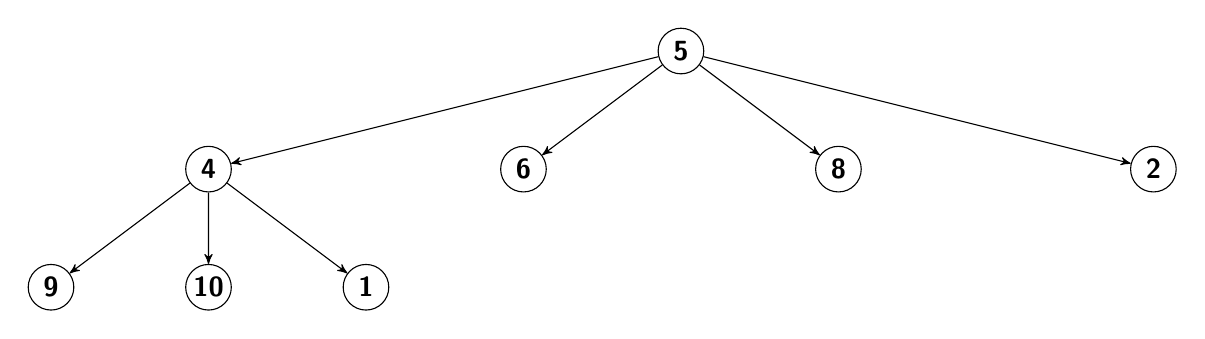
\begin{tikzpicture}[->,>=stealth',level/.style={sibling distance = 4cm/#1,
            level distance = 1.5cm}] 
            \node [arn_n] {5} % ROOT
            child{ node [arn_n] {4} 
                child{ node [arn_n] {9}}
                child{ node [arn_n] {10}}                            
                child{ node [arn_n] {1}}                            
            }
            child{ node [arn_n] {6}}
            child{ node [arn_n] {8}}
            child{ node [arn_n] {2}}
            ; 
        \end{tikzpicture}
        
        \item Looking at the tree you have drawn, how many leaves and nodes are present? 

        6 leaves, 8 nodes, 2 of which are internal.
        
        \item Examine your tree and find both the root and the node with the value 4. For both nodes, list the following attributes: depth, height of subtrees, number of siblings, number of children. 

        Root Node: \{ depth: 0, height of subtrees: [2, 1, 1, 1], number of siblings: 0, number of direct children: 4, descendants: 7 \}

        Node(4) \{ depth: 1, height of subtrees: [1, 1, 1, 0], number of siblings: 3, number of direct children: 3, descendants: 3 \}
        
        \item Insert 6 more random elements into your tree and relist any of the above attributes that have changed.

        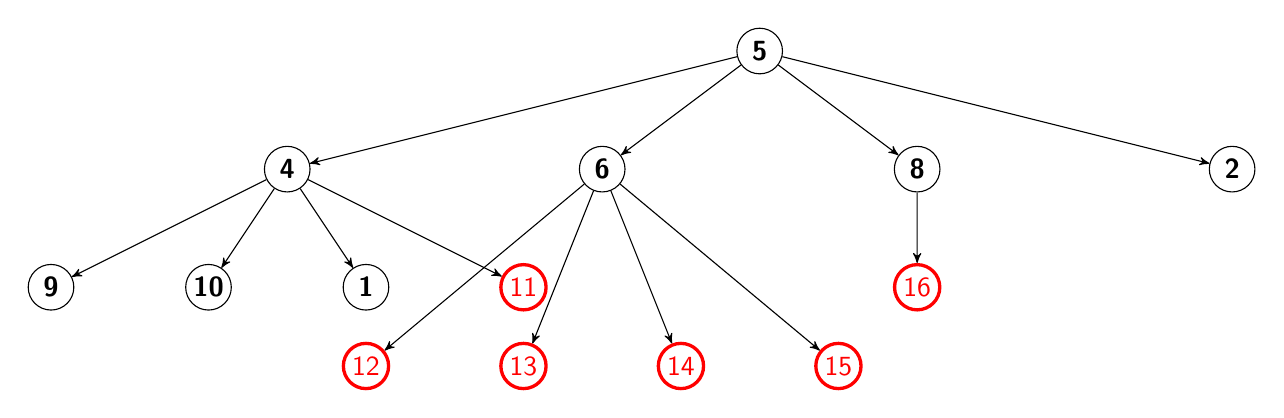
\begin{tikzpicture}[->,>=stealth',level/.style={sibling distance = 4cm/#1,
            level distance = 1.5cm}] 
            \node [arn_n] {5} % ROOT
            child{ node [arn_n] {4} 
                child[sibling distance = 2cm]{ node [arn_n] {9}}
                child[sibling distance = 2cm]{ node [arn_n] {10}}                            
                child[sibling distance = 2cm]{ node [arn_n] {1}}  
                child[sibling distance = 2cm]{ node [arn_r] {11}}                         
            }
            child{ node [arn_n,] {6}
                child[level distance = 2.5cm]{ node [arn_r] {12}}
                child[level distance = 2.5cm]{ node [arn_r] {13}}
                child[level distance = 2.5cm]{ node [arn_r] {14}}
                child[level distance = 2.5cm]{ node [arn_r] {15}}
            }
            child{ node [arn_n] {8}
                child{ node [arn_r] {16}}
            }
            child{ node [arn_n] {2}}
            ; 
        \end{tikzpicture}

        Root Node: \{ depth: 0, height of subtrees: [2, 2, 2, 1], number of siblings: 0, number of direct children: 4, descendants: 13 \}

        Node(4) \{ depth: 1, height of subtrees: [1, 1, 1, 1], number of siblings: 3, number of direct children: 4, descendants: 4 \}
        
        \item Would the structure (shape of the tree and not values of the nodes) of the k-ary tree you've drawn change at all if the elements were inserted in sorted order? Explain why or why not.

        No. K-ary trees are not sorted trees.
    \end{enumerate}
    
    \section{Doubly Linked Lists}
    
    \begin{enumerate}
    
        \item Describe an algorithm to count the number of sets of three adjacent nodes whose sum is equal to 0.\\
        Set a counter to 0. Set a pointer to the second element of the list. Check whether the sum of the node pointed to, its predecessor, and its successor is 0 and increment the counter if true. Set the pointer to the next element of the list and repeat until the successor is null.
        
        \item For a doubly linked list with n elements, how much additional memory is going to be used compared to a singly linked list?\\
        n pointers will be allocated
    
    \end{enumerate}
    
    \section{Stacks and Queues}
    \begin{enumerate}

        \item Is a linked list the best underlying structure to implement a queue with? Justify your answer. 

        Linked lists are a convenient underlying structure, but there is no true best when it comes to queues. So long as your implementation offers constant time operations and minimal space requirements.
        
        \item Is a linked list the best underlying structure to implement a stack with? Justify your answer. 

        Linked lists are a convenient underlying structure, but there is no true best when it comes to queues. So long as your implementation offers constant time operations and minimal space requirements.
        
        \item Would a stack or queue be more efficient for the following:
        \begin{enumerate}
            \item An undo button in a text editor\\
            stack
            \item A web server\\
            queue
            \item A breadth-first search\\
            queue
            \item A depth-first search\\
            stack
        \end{enumerate}
    \end{enumerate}
    
    \label{r:lastpage}
    
    \end{document}
        
    
